\documentclass[10pt,a4paper]{article}
\usepackage[margin=2cm,top=1.6cm,bottom=1.8cm]{geometry}
\usepackage[T1]{fontenc}
\IfFileExists{lmodern.sty}{\usepackage{lmodern}}{\usepackage{mathptmx}}
\usepackage{microtype,booktabs,graphicx,xcolor,tabularx,amsmath,enumitem,float}
\usepackage[font=small,labelfont=bf,skip=3pt]{caption}
\usepackage[colorlinks,urlcolor=blue!60!black,linkcolor=black,citecolor=black]{hyperref}
\setlist{nosep,leftmargin=1.2em}
\setlength{\parskip}{3pt}
\setlength{\parindent}{0pt}
% ------------------------------------------------------------------ set these
\newcommand{\repourl}{\textcolor{red}{https://github.com/TODO/bm25-vs-neural}}
% -----------------------------------------------------------------------------
\IfFileExists{tables/macros.tex}{% generated by scripts/make_report_macros.py - do not edit
\newcommand{\corpusN}{\textcolor{red}{??}}
\newcommand{\corpusPrimary}{\textcolor{red}{??}}
\newcommand{\corpusInCat}{\textcolor{red}{??}}
\newcommand{\corpusFiltered}{\textcolor{red}{??}}
\newcommand{\corpusDup}{\textcolor{red}{??}}
\newcommand{\corpusWithdrawn}{\textcolor{red}{??}}
\newcommand{\corpusSha}{\textcolor{red}{??}}
\newcommand{\sciDiff}{\textcolor{red}{??}}
\newcommand{\sciOverlap}{\textcolor{red}{??}}
\newcommand{\sciCritI}{\textcolor{red}{??}}
\newcommand{\sciCritII}{\textcolor{red}{??}}
\newcommand{\sciPys}{\textcolor{red}{??}}
\newcommand{\sciBMplain}{\textcolor{red}{??}}
\newcommand{\sciBM}{\textcolor{red}{??}}
\newcommand{\sciEfive}{\textcolor{red}{??}}
\newcommand{\sciSpec}{\textcolor{red}{??}}
\newcommand{\sciHybE}{\textcolor{red}{??}}
\newcommand{\sciHybS}{\textcolor{red}{??}}
\newcommand{\reuDiff}{-0.0026}
\newcommand{\reuOverlap}{96.8}
\newcommand{\reuRatio}{1.900}
\newcommand{\reuDocs}{10{,}788}
\newcommand{\reuQueries}{100}
\newcommand{\truncEfive}{\textcolor{red}{??}}
\newcommand{\encMinEfive}{\textcolor{red}{??}}
\newcommand{\medTokEfive}{\textcolor{red}{??}}
\newcommand{\truncSpec}{\textcolor{red}{??}}
\newcommand{\encMinSpec}{\textcolor{red}{??}}
\newcommand{\medTokSpec}{\textcolor{red}{??}}
\newcommand{\gpuName}{\textcolor{red}{??}}
\newcommand{\bmIndexSec}{\textcolor{red}{??}}
\newcommand{\bmIndexMB}{\textcolor{red}{??}}
\newcommand{\bmMs}{\textcolor{red}{??}}
\newcommand{\bmVocab}{\textcolor{red}{??}}
\newcommand{\poolSize}{\textcolor{red}{??}}
\newcommand{\poolPerQ}{\textcolor{red}{??}}
\newcommand{\poolPrio}{\textcolor{red}{??}}
\newcommand{\anchorsFound}{\textcolor{red}{??}}
\newcommand{\anchorsMissing}{\textcolor{red}{??}}
\newcommand{\kappaLin}{\textcolor{red}{??}}
\newcommand{\kappaQuad}{\textcolor{red}{??}}
\newcommand{\nDouble}{\textcolor{red}{??}}
\newcommand{\ovBE}{\textcolor{red}{??}}
\newcommand{\ovBEId}{\textcolor{red}{??}}
\newcommand{\ovBEPara}{\textcolor{red}{??}}
\newcommand{\ovBS}{\textcolor{red}{??}}
\newcommand{\ovBSId}{\textcolor{red}{??}}
\newcommand{\ovBSPara}{\textcolor{red}{??}}
\newcommand{\ovES}{\textcolor{red}{??}}
\newcommand{\ovESId}{\textcolor{red}{??}}
\newcommand{\ovESPara}{\textcolor{red}{??}}
}{}
\IfFileExists{tables/fin_macros.tex}{\newcommand{\finStatus}{PRELIMINARY: 325 annotator conflicts are not yet adjudicated}
\newcommand{\finKappaLin}{0.760}
\newcommand{\finKappaQuad}{0.829}
\newcommand{\finKappaBin}{0.795}
\newcommand{\finExact}{0.757}
\newcommand{\finConflicts}{325}
\newcommand{\finZeroThree}{21}
\newcommand{\finCross}{134}
\newcommand{\finPairs}{1339}
\newcommand{\finOnlyBM}{116--146}
\newcommand{\finOnlyE}{140--174}
\newcommand{\finBoth}{96--115}
\newcommand{\finSensFirst}{100}
\newcommand{\finSensN}{500}
\newcommand{\finSensTopOrder}{93}
\newcommand{\finBoundHybE}{0.657--0.798}
\newcommand{\finBoundBM}{0.614--0.765}
\newcommand{\finBoundE}{0.639--0.774}
}{\newcommand{\finStatus}{tables missing}}
\newcommand{\inputor}[2]{\IfFileExists{#1}{\input{#1}}{#2}}
% defined only in preliminary mode; in final mode these show "?" until the prose is revised
\providecommand{\finSensN}{\textcolor{red}{?}}\providecommand{\finSensFirst}{\textcolor{red}{?}}
\providecommand{\finSensTopOrder}{\textcolor{red}{?}}\providecommand{\finBoundHybE}{\textcolor{red}{?}}
\newcommand{\pending}[1]{\textcolor{red!70!black}{[#1]}}

\begin{document}
\begin{center}
{\Large\bfseries Domain-Specific Search: BM25 vs.\ Neural Retrieval on Technical Documents}\\[3pt]
{\large Final Report \;|\; Information Retrieval \;|\; Group 10}\\[4pt]
\begin{tabular}{llll}
Surajsinh Patil & 2025H1030058P & Tejas Mahajan & 2025H1030057P\\
Swayam Kumud & 2025H1030063P & Saksham Singhal & 2025H1030208P
\end{tabular}\\[3pt]
\textbf{Repository:} \repourl\\[6pt]
\fcolorbox{red!60!black}{red!5}{\parbox{0.92\linewidth}{\small\textbf{Status: \finStatus.}
Every cs.CR effectiveness number below is shown as a range: the value with all unresolved
conflicts at the lower grade, and with all of them at the higher grade. These two runs are a sensitivity
check, not bounds (nDCG is not monotone in the grades). Exact bounds over all adjudications, and
results for random adjudications, are given in Table~\ref{tab:fsens}. The SciFact numbers (Section~\ref{sec:sci}) only validate the
implementation and are not cs.CR results.}}
\end{center}

\section{Introduction}
Dense retrievers trained on general web data are often assumed to beat lexical retrieval. We test
this on technical text where exact strings matter: computer-security abstracts from arXiv (cs.CR),
which are full of identifiers (CVE numbers, protocol versions), homonyms (\emph{oracle},
\emph{poisoning}, \emph{fingerprinting}) and conditions such as exclusions and date limits.
We compare our identifier-aware BM25, two dense models used without fine-tuning (E5-base-v2 and
SPECTER2), and their Reciprocal Rank Fusion hybrids. Research questions:
\textbf{RQ1} Does a dense retriever beat BM25 overall?
\textbf{RQ2} How does this depend on the query type?
\textbf{RQ3} Does the science-specific SPECTER2 beat the general E5?
\textbf{RQ4} Does a hybrid beat both of its components?
\textbf{RQ5} How sensitive is BM25 to $k_1$, $b$ and tokenisation?

\section{Related work}
BM25 \cite{robertson} remains a strong zero-shot baseline: in BEIR \cite{beir} it beat many dense
models outside their training domain. E5 \cite{e5} is trained contrastively on large weakly
supervised pair data and then fine-tuned. SPECTER2 \cite{specter2} is trained on scientific
citation data, with task adapters for proximity and ad-hoc search. RRF \cite{rrf} fuses ranked
lists using ranks only. Bruch et al.\ \cite{bruch} compare RRF with convex score combination.
Dense models are known to handle negation poorly \cite{nevir}. Our design for significance tests
follows Smucker et al.\ \cite{smucker}; for assessor disagreement it follows Voorhees \cite{voorhees}.

\section{Data, queries and systems}
\textbf{Corpus.} We use all \corpusN{} arXiv papers with cs.CR as primary or cross-listed category
and a first version in 2016--2025. Withdrawn papers and duplicate titles are removed and LaTeX is
cleaned (SHA-256 \texttt{\corpusSha\ldots}). A document is its title plus abstract.
\textbf{Queries.} 50 queries, 10 per category: exact identifier (e.g.\ ``Spectre variant~1 bounds check
bypass (CVE-2017-5753)''), homonym (``padding oracle attacks on CBC mode''), negation (``anonymous
communication systems that are \emph{not} based on Tor''), time constraint (``attacks on TLS~1.3
published after its 2018 standardisation'') and paraphrase (``copying a deployed model by repeatedly
querying its prediction interface''). Each query has a description and written relevance criteria.
\textbf{Systems.} (1)~BM25 ($k_1{=}1.2$, $b{=}0.75$) with an identifier-aware analyzer. It keeps
\texttt{cve-2021-44228} or \texttt{tls1.3} as single tokens and also indexes their parts;
Lucene's stopwords are removed (including ``not'') and the Porter stemmer is applied.
(2)~E5-base-v2 and (3)~SPECTER2 (proximity adapter for documents, ad-hoc query adapter for queries),
both with exact cosine search. (4, 5)~RRF ($k{=}60$, top 100 of each run) of BM25 with E5 and with
SPECTER2. Nothing was tuned on our queries.

\section{Evaluation protocol}
\textbf{Pooling and judging.} The top 10 of all five runs form the pool: \finPairs{} query--document
pairs, about 27 per query. Every query was judged independently by two of the four authors, with the
six annotator pairs spread evenly. The judging pages showed no system names or ranks, and showed dates
only for time queries. Grades: 0 not relevant, 1 on topic but does not answer the query or breaks a
condition, 2 relevant, 3 highly relevant. All 2{,}678 judgments were collected and audited: none is
missing, duplicated or outside the pool.
\textbf{Agreement.} Weighted Cohen's $\kappa$ = \finKappaLin{} (linear) and \finKappaQuad{}
(quadratic); $\kappa$ on binary relevance (grade $\geq 2$) = \finKappaBin{}; exact agreement
\finExact{}. This meets the protocol's target of $\kappa\geq 0.6$. \finConflicts{} pairs conflict:
\finZeroThree{} are 0 vs 3, and \finCross{} fall on opposite sides of the relevance line. By protocol,
conflicts are adjudicated by the team before the qrels are frozen.
\textbf{Metrics.} The primary metric is nDCG@10 with gain equal to the grade. P@5, MRR@10 and MAP@10
use grade $\geq 2$. Unjudged documents count as non-relevant; Hole@10 reports how often they occur.
Our metric code matches \texttt{trec\_eval} (via \texttt{pytrec\_eval}) on every query of every run,
with a maximum difference of $3\times10^{-16}$.
\textbf{Significance.} Paired randomisation tests over queries (100{,}000 permutations) on nDCG@10 for
all 10 system pairs, with Holm--Bonferroni correction. Per-category results come with 95\% bootstrap
CIs and are exploratory, since each category has only 10 queries.

\section{Results}
\subsection{Validation of the implementation (SciFact)}\label{sec:sci}
This is not a cs.CR result. On BEIR SciFact (300 queries) with the same settings as Pyserini, our BM25
differs from Lucene by $\Delta$nDCG@10 = \sciDiff{} and shares \sciOverlap\% of its top-10 documents.
On the same collection E5 (\sciEfive) beats BM25 (\sciBM) significantly ($p_{\text{Holm}}$ =
\sciPBmtwofiveEfive), while SPECTER2 (\sciSpec) does not.

\subsection{Main results on cs.CR}
\inputor{tables/fin_main.tex}{}
\inputor{tables/fin_sig.tex}{}
Tables~\ref{tab:fmain} and~\ref{tab:fsig} show that Hole@10 is 0 for every system: every document in
every top 10 was judged. Table~\ref{tab:fsens} shows how far adjudication can move the comparisons.
We enumerated every way of resolving each conflict to one of its two submitted grades, which gives exact
ranges of the mean differences. We also drew \finSensN{} random adjudications.
\inputor{tables/fin_sens.tex}{}
\textbf{RQ1:} E5 and BM25 are statistically indistinguishable overall (difference 0.006--0.020 in
favour of E5, $p_{\text{Holm}}=1$). The sign of the difference depends on adjudication, and the
difference is significant in none of the random adjudications. The data give no support for the claim
that a general dense model beats BM25 on this collection.
\textbf{RQ3:} SPECTER2 is the weakest system, significantly worse than BM25, E5 and both hybrids
(0.105--0.164 below BM25 and E5). No adjudication can reverse the direction of these four differences,
and they are significant in 99--100\% of random adjudications. A deliberately adversarial adjudication
can make them non-significant, however, so this conclusion is final only after the real adjudication.
SPECTER2's citation-based training does not transfer to short ad-hoc queries.
\textbf{RQ4:} BM25+E5 has the highest mean nDCG@10 under both fallback runs (0.699--0.766) and in
\finSensFirst\% of random adjudications (exact range over all adjudications \finBoundHybE), but its gains
over BM25 (+0.035--0.042) and E5 (+0.021--0.029) are not significant after correction. Fusing BM25 with
SPECTER2 recovers most of SPECTER2's loss but does not beat BM25.

\subsection{By query type (RQ2, exploratory)}
\inputor{tables/fin_cat.tex}{}
\IfFileExists{figures/fin_per_category.pdf}{\begin{figure}[t]\centering
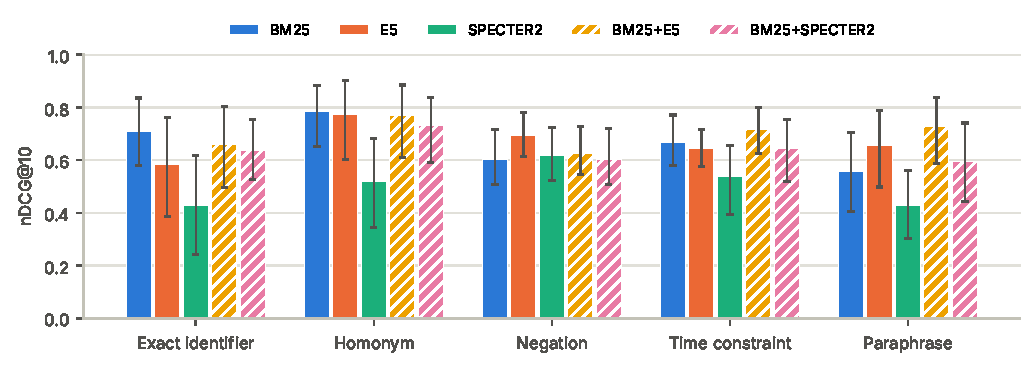
\includegraphics[width=\linewidth]{figures/fin_per_category.pdf}
\caption{nDCG@10 per category with 95\% bootstrap CIs, lower bound (hatched = hybrids). Exploratory.}
\label{fig:fcat}\end{figure}}{}
Under both fallback runs (Table~\ref{tab:fcat}), BM25 leads on \emph{exact identifiers} (0.708--0.825
vs.\ 0.583--0.722 for E5), while E5 leads on \emph{paraphrases} (0.656--0.723 vs.\ 0.558--0.621) and
\emph{negation} (0.676--0.692 vs.\ 0.562--0.601). BM25+E5 is best on paraphrase and time queries.
On homonyms, BM25, E5 and BM25+E5 are all high (above 0.77). With 10 queries per category the CIs
overlap widely, so these are hypotheses for follow-up rather than findings. Within-category tests (Holm-corrected within each category) find only a few significant
differences, none of them in both fallback runs: BM25+E5 over BM25 on paraphrases (lower bound), and
SPECTER2 below each of the other four systems on homonyms (upper bound).

\subsection{Error analysis}
\inputor{tables/fin_g1.tex}{}
\textbf{Conditions are ignored.} On negation queries, 76--81\% of BM25's top 10 are graded 1, mostly
papers that break the exclusion. The figure is 59--63\% for E5 and 68--74\% for BM25+E5
(Table~\ref{tab:fg1}). BM25 removes ``not'' as a stopword. For ``anonymous communication systems that
are not based on Tor'', nine of BM25's top 10 were graded 1 by both annotators, the grade the
relevance criteria give to papers about Tor itself. Six of E5's top 10 were graded 2 or 3 by both
annotators. On time queries, 39--58\% of each system's top 10 is graded 1. Counting from
first-version dates, 30--38\% of each system's top 10 breaks the date condition; a rule-based date
filter (stretch goal S2) removes all of these.
\textbf{Paraphrases defeat lexical matching.} For ``programs that lock a victim's files and demand
payment to unlock them'', BM25 ranks four non-relevant documents in its top five, while E5 returns
ransomware papers that both annotators graded 2--3.
\textbf{The two systems complement each other.} Of the relevant documents in the BM25 and E5 top 10s,
\finBoth{} are found by both, \finOnlyBM{} only by BM25 and \finOnlyE{} only by E5. This explains why
fusion helps even though neither component is better overall. Full examples are in
\texttt{deliverables/*/analysis/error\_analysis.md}.

\subsection{Efficiency}
\inputor{tables/efficiency_prelim.tex}{}
All numbers are measured from the run logs (Table~\ref{tab:eff}). BM25 builds its index in 20\,s on one
CPU into 29\,MB and answers in 1.6\,ms. Each dense index is 116\,MB (4$\times$ larger) and takes about
3\,min of T4 GPU time. Dense queries take 17--30\,ms, mostly query encoding; exact search alone takes
6--7\,ms. BM25+E5 therefore buys its effectiveness at roughly 12$\times$ the query cost of BM25.

\subsection{BM25 sensitivity (RQ5)}
\pending{Blocked until the qrels are frozen: \texttt{bm25\_sweep.py} (with 5-fold cross-validation,
so no tuning on the test queries is reported as a test score) and \texttt{tokenizer\_ablation.py} need
the corpus and run on Kaggle.}

\section{Limitations}
(1) The results are preliminary until the \finConflicts{} conflicts are adjudicated. The system order is
the same in \finSensTopOrder\% of random adjudications, but significance is guaranteed only for the real one. (2) There are 50 queries, 10 per category, so category effects are
exploratory. (3) The pool contains only the top 10 of five systems. Hole@10 is 0 for these systems, but
recall-oriented metrics, and any system outside the pool, would be biased. (4) No relevant document
(grade $\geq 2$) was found for one query (AES-GCM nonce reuse); it counts for every system, and removing
it does not change the system order. (5) The authors wrote the queries and judged them. (6) The dense
models may have seen arXiv abstracts during pre-training. (7) A grade of 1 earns nDCG gain, so systems
partly get credit for documents that break a condition; an exploratory strict variant (no gain for
grade 1, \texttt{sNDCG@10} in the result files) gives the same system order, except that BM25 and
BM25+SPECTER2 tie under the upper bound.

\section{Conclusions}
On security abstracts, a general dense retriever used without fine-tuning does not beat a careful BM25
overall. The science-specific SPECTER2 is clearly worse than both. BM25 and E5 fail on different
queries: BM25 on paraphrases and negation, E5 on exact identifiers. Their RRF fusion scores highest
under every adjudication we sampled, but its gain over the better component is not significant with 50 queries, and it
costs about 12$\times$ the query time of BM25. Every system largely ignores exclusions and date limits;
handling them explicitly (S2) is more promising than switching models.

\section*{Contribution matrix}
\begin{tabularx}{\linewidth}{@{}l X@{}}
\toprule
Member & Components\\
\midrule
Surajsinh Patil & \pending{fill in}\\
Tejas Mahajan & \pending{fill in}\\
Swayam Kumud & \pending{fill in}\\
Saksham Singhal & \pending{fill in}\\
All & Query writing; relevance judging (about 670 judgments each); adjudication\\
\bottomrule
\end{tabularx}

\begin{thebibliography}{99}\small
\bibitem{robertson} S.~Robertson, H.~Zaragoza. The Probabilistic Relevance Framework: BM25 and Beyond. \emph{Found.\ Trends IR}, 2009.
\bibitem{beir} N.~Thakur et al. BEIR: A Heterogeneous Benchmark for Zero-shot Evaluation of Information Retrieval Models. \emph{NeurIPS Datasets and Benchmarks}, 2021.
\bibitem{e5} L.~Wang et al. Text Embeddings by Weakly-Supervised Contrastive Pre-training. arXiv:2212.03533, 2022.
\bibitem{specter2} A.~Singh et al. SciRepEval: A Multi-Format Benchmark for Scientific Document Representations. \emph{EMNLP}, 2023.
\bibitem{rrf} G.~V.~Cormack, C.~L.~A.~Clarke, S.~Buettcher. Reciprocal Rank Fusion Outperforms Condorcet and Individual Rank Learning Methods. \emph{SIGIR}, 2009.
\bibitem{bruch} S.~Bruch, S.~Gai, A.~Ingber. An Analysis of Fusion Functions for Hybrid Retrieval. \emph{ACM TOIS}, 2023.
\bibitem{nevir} O.~Weller, D.~Lawrie, B.~Van Durme. NevIR: Negation in Neural Information Retrieval. \emph{EACL}, 2024.
\bibitem{smucker} M.~D.~Smucker, J.~Allan, B.~Carterette. A Comparison of Statistical Significance Tests for Information Retrieval Evaluation. \emph{CIKM}, 2007.
\bibitem{voorhees} E.~M.~Voorhees. Variations in Relevance Judgments and the Measurement of Retrieval Effectiveness. \emph{Inf.\ Process.\ Manage.}, 2000.
\end{thebibliography}
\end{document}
